\documentclass[12pt]{article}


\title{Unixcrypt Multi-block Analysis}
\date{Aug 2019}
\author{Charlie Gerrie}
\usepackage[utf8]{inputenc}


\usepackage{amsthm}
\usepackage{amsmath}
\usepackage{yfonts}
\usepackage{amssymb}
\usepackage{fullpage}
\usepackage{mathtools}
\usepackage{tikz}
\usepackage{graphicx}
\usepackage{subcaption}
\usepackage{float}
\usepackage{pgf}
\usepackage{url}
\usetikzlibrary{arrows}
\DeclarePairedDelimiter\ceil{\lceil}{\rceil}
\DeclarePairedDelimiter\floor{\lfloor}{\rfloor}
\pagestyle{empty}

\newtheorem{theorem}{Theorem}%[section]

\newtheorem{lemma}{Lemma}%[section]

\newtheorem{proposition}{Proposition}%[section]

\newtheorem{corollary}{Corollary}%[section]

\theoremstyle{definition}
\newtheorem{definition}{Definition}%[section]
 
\theoremstyle{remark}
\newtheorem{remark}{Remark}%[section]

\theoremstyle{remark}
\newtheorem{example}{Example}%[section]

\pagenumbering{gobble}
% TODO SHOULD I HAVE PAGE NUMBERS?

\begin{document}

%TITLE PAGE%
\maketitle
\newpage

% TODO ABSTRACT PAGE
\begin{center}{\textbf{Abstract}}\end{center}
\newpage

\section{Background}

\subsection{The Cipher}
\par
The unixcrypt cipher key is defined by two permutations $\mathbb{Z}_{256}$ denoted by the characters $\tau$ and $\sigma$. They are both permutations on the 256-element set of all bytes. $\tau$ must be a 256-cycle. $\sigma$ must be self-inverse ($\sigma^2=\texttt{id}$) and have no fixed points ($\sigma(x)\neq x$), or in other words it must be entirely composed of 2-cycles.
% TODO put in equations

\par
For the rest of this paper the symbols $\tau$ and $\sigma$ will be used interchangeably with the words tau and sigma.
% explain calling it tau not \tau

\par
Much of the discussion to come will be referring to \emph{wires}. These will be referring to preimage-image pairs in a given permutation. The wire's preimage will also be referred to as its \emph{startpoint} and its image will be referred to as its \emph{endpoint}. 
% explain wires analogy
% TODO example
% TODO explain where it comes from
\begin{definition}[Wire]
	TODO restate that
\end{definition}

\par
When using the cipher we will consider two bodies of text, the plaintext and the ciphertext. Both represent sequences of characters, but will in practice be treated as sequences of numbers from $0$ to $255$. The ciphertext will be produced from the plaintext by the algorithm.
% define plaintext and ciphertext?
% QUESTION is this necessary?

\par The $i$th plain text $p_i$, where $i=256 j + k$ for $0\leq k < 256$, is encoded by
\begin{equation}
	\label{ciphereq}
	c_i = \kappa^{-k} \tau^{-j} \sigma \tau^j \kappa^k p_i
\end{equation}
where $c_i$ is the $i$th ciphertext, and $\kappa$ is the successor function. Exponentiation represents repeated function application.


\par
It should be noted that this cipher is symmetric-key, meaning it uses the same key for encryption and decryption. Further, the encryption and decryption processes are the exact same. This follows from equation (\ref{ciphereq}) and the fact that $\sigma^2=\texttt{id}$.
% TODO proof
% TODO refer to sigma squared = 1 equation

\par
Notice that the exponent on tau is only incremented when $j$ is incremented. This happens every 256 characters. These 256 character long sections of text which share the same $j$ are referred to as blocks.
% blocks
\begin{definition}[Block]
	TODO restate that
\end{definition}

\par
Usually we define $\sigma_j = \tau^{-j} \sigma \tau^j$. This combines both the sigma and tau parts of the key into one, giving us a single permutation for encoding the $j$th block. This will be important for using the information from the single-block analysis. Note that $\sigma_0 = \sigma$.
\begin{definition}[Block Key]
	TODO restate that
	\begin{equation}
		\label{blockeq}
		\sigma_j = \tau^{-j} \sigma \tau^j
	\end{equation}
\end{definition}
% sigma_j and sigma_j hat

\subsection{Single-Block Analysis}
\par
Previous work on this cipher has produced a method of single-block analysis [1]. This looks at each block individually and tries to find, or in practice approximate, the block keys for each block. Thus, we obtain approximations of each block key $\sigma_j$, which we will denote $\hat{\sigma}_j$. 
% single-block analysis
% TODO outline more!
% TODO REFERENCE
\par
Each block only consists of 256 characters, so on average every wire is used just once.
% TODO finish
% QUESTION rational for 
In practice what this means is that the single-block analysis can successfully reproduce about half of the wires in each block key. It also makes a small number of incorrect guesses, and leaves the rest of the wires unguessed. This last part is insignificant when the single-block analysis is performed by itself, but to perform the multi-block analysis we will need the block key approximations to be complete permutations so we can perform calculations with them. Thus, to "fill out" the permutations we assign the unguessed wires at random. This can be done efficiently with a Fisher-Yates shuffle.
% success

\section{Finding Tau}
\subsection{Generating the Coincidences Distribution}

\par
The basic goal of the multi-block analysis is to use the block key approximations provided by the single-block analysis to reconstruct the original key. We begin by finding tau.
% how we plan to use sigma hats

\par
We will use some custom notation for wires and multisets. A wire from $a$ to $b$ will be denoted $(a,b)$. A multiset can be defined using normal set builder notation except with double brackets.
% TODO wire and multiset notation
% QUESTION multiset citation?
\par
Figure \ref{ladderfig} shows a commutative diagram derived from equation (\ref{blockeq}). Of particular note is the equivalence of $\tau$ and $\sigma_1 \tau \sigma^{-1}_0$, marked in red and blue respectively. Thus, if we conjecture that $(a,b)$ is a wire in $\tau$ then it must also be a wire in $\sigma_1 \tau \sigma^{-1}_0$. But the wire in $\sigma_1 \tau \sigma^{-1}_0$ is really three wires: a wire $(a,\sigma_1(a))$ in $\sigma_1$, a wire $(\sigma_1(a),\sigma_0(b))$ in $\tau$, and a wire $(\sigma_0(b), b)$ in $\sigma^{-1}_0$. Thus, if $(a,b)$ is a wire in $\tau$ then $(\sigma_1(a),\sigma_0(b))$ must also be a wire in $\tau$. In general, all wires $(\sigma_{i+1}(a),\sigma_i(b))$ must be in $\tau$. Thus, the \emph{wire consequences} of $(a,b)$ are all the wires that must also be in $\tau$ if $(a,b)$ is.

% explain ladder diagram
\begin{figure}[h!]
	\centering
	\caption{}
	\label{ladderfig}
	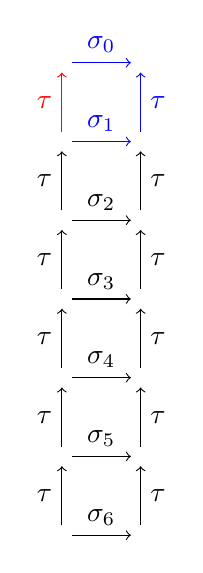
\begin{tikzpicture}[node distance=10pt]
		\foreach \i in {0,...,6} {
			\node (L\i) at (0,-\i) {};
			\node (R\i) at (1,-\i) {};
		}
		\foreach \i in {0,...,5} {
			\node (BL\i) at (0,-\i-1) {};
			\node (BR\i) at (1,-\i-1) {};
		}
		\draw [red, arrows={->}] (BL0) edge node[left] {$\tau$} (L0);
		\draw [blue, arrows={->}] (L0) edge node[above] {$\sigma_0$} (R0);
		\draw [blue, arrows={->}] (BR0) edge node[right] {$\tau$} (R0);
		\draw [blue, arrows={->}] (L1) edge node[above] {$\sigma_1$} (R1);
		\foreach \i in {2,...,6} {
			\draw [->] (L\i) edge node[above] {$\sigma_\i$} (R\i);
		}
		\foreach \i in {1,...,5} {
			\draw [->] (BL\i) edge node[left] {$\tau$} (L\i);
			\draw [->] (BR\i) edge node[right] {$\tau$} (R\i);
		}
	\end{tikzpicture}
\end{figure}
\begin{definition}[Wire Consequences]
	For a wire $(a,b)$, we have
	\begin{equation}
		\texttt{conseq}(a,b)=\{\{(\hat{\sigma}_i(a), \hat{\sigma}_{i+1}(b)) : 0\leq i <N-1\}\}\end{equation}
	where $N$ is the number of sigma hats. This is a multiset.
\end{definition}





\par
TODO Explain why coincidences






\begin{definition}[Wire-to-wire Coincidences]
	If we consider two wires $(a,b)$ and $(c,d)$, then we have
	\begin{equation}
		\label{coinceq}
		\texttt{coinc}(a,b,c,d)=\sum^{255}_{i=0} \sum^{255}_{j=0} \texttt{conseq}(a,b)_{i,j} \texttt{conseq}(c,d)_{i,j}
	\end{equation}
	where $\texttt{conseq}(a,b)_{i,j}$ is the multiplicity of the wire $(i,j)$ in the consequences of $(a,b)$.
% TODO equation
	This is a count of all the possible pairs of similar elements in the two wires consequence multisets. 
\end{definition}
\begin{figure}[h!]
	\centering
	\caption{}
	\label{coincfig}
	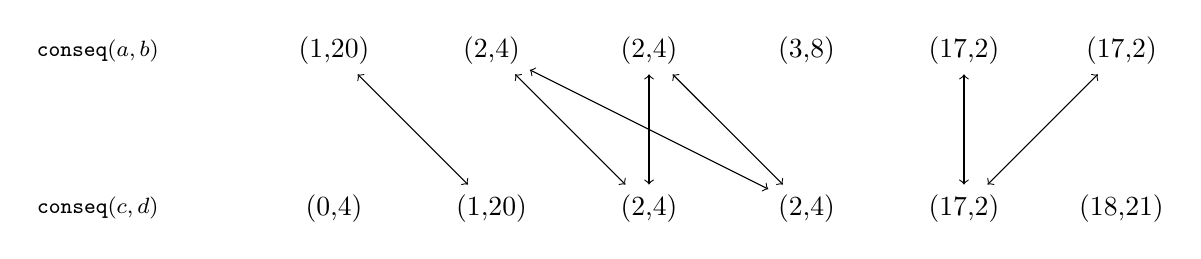
\begin{tikzpicture}
		\node (cons1) at (-3,0) {\begin{footnotesize}$\texttt{conseq}(c,d)$\end{footnotesize}};
		\node (cons2) at (-3,2) {\begin{footnotesize}$\texttt{conseq}(a,b)$\end{footnotesize}};	
	
		\node (T1) at (0,0) {(0,4)};
		\node (T2) at (2,0) {(1,20)};
		\node (T3) at (4,0) {(2,4)};
		\node (T4) at (6,0) {(2,4)};
		\node (T5) at (8,0) {(17,2)};
		\node (T6) at (10,0) {(18,21)};
		\node (B1) at (0,2) {(1,20)};
		\node (B2) at (2,2) {(2,4)};
		\node (B3) at (4,2) {(2,4)};
		\node (B4) at (6,2) {(3,8)};
		\node (B5) at (8,2) {(17,2)};
		\node (B6) at (10,2) {(17,2)};
		
		\draw [<->] (T2) -- (B1);
		\draw [<->] (T3) -- (B2);
		\draw [<->] (T4) -- (B2);
		\draw [<->] (T3) -- (B3);
		\draw [<->] (T4) -- (B3);
		\draw [<->] (T5) -- (B5);
		\draw [<->] (T5) -- (B6);
	\end{tikzpicture}
\end{figure}
% TODO FIGURE arrows for pairing up

\par
Figure \ref{coincfig} shows how we count the possible pairs. This example would be expressed as an expansion of equation (\ref{coinceq}) as follows:
\begin{equation}
\begin{split}
	\texttt{coinc}(a,b,c,d) =& \sum^{255}_{i=0} \sum^{255}_{j=0} \texttt{conseq}(a,b)_{i,j} \texttt{conseq}(c,d)_{i,j} \\ =& \texttt{conseq}(a,b)_{1,20} \texttt{conseq}(c,d)_{1,20} + \texttt{conseq}(a,b)_{2,4} \texttt{conseq}(c,d)_{2,4} \\ & + \texttt{conseq}(a,b)_{17,2} \texttt{conseq}(c,d)_{17,2} \\  = & (1)(1) + (2)(2) + (2)(1) \\  = & 7
\end{split}
\end{equation}
with all other terms in the sums evaluating to zero.

\par
Finally, it should be noted that wire-to-wire coincidences are always non-negative integers.


% explain figure

\begin{definition}[Coincidences Distribution]
	Given a wire, we can define a discrete distribution of the value of the wire-to-wire coincidences between that wire and another randomly chosen wire.
\end{definition}
% TODO equation?
% TODO FIGURE example histogram? 
\par
Here is an example the coincidences distribution for a wire (75,29), encoding the probability of each number of wire-to-wire coincidences between (75,29) and a randomly chosen wire (c,d).
\begin{center}
\begin{tabular}{|c|c|c|c|c|}
\hline
$X$ & 0 & 1 & 2 & ... \\
\hline 
$P(\texttt{coinc}(75,29,c,d)=X)$ & 0.933 & 0.0648 & 0.00224 & ... \\

\hline
\end{tabular}
\end{center}
% TODO facts and general shape
Notice that it is very likely that the number of wire-to-wire coincidences is 0, and that the probability falls of sharply as the number of coincidences increases. Note that in practice we generate this distribution by sampling the wire-to-wire coincidences between the given wire $(a,b)$ and wires $(c,d)$ that satisfy the following conditions: $a\neq b$ and $c\neq d$ because tau is a 256-cycle and cannot have fixed points, and $a\neq c$ and $b \neq d$ because then they would be mutually exclusive. There are 64771 such wires. 

\par
Now to reconstruct tau, we need to find all 256 of its wires. To do this, we calculate the coincidences distribution for all possible wires, of which there are $256 \times 255$ since wires in tau cannot connect to themselves. Then for all 256 wire start-points, we will pick the best end-point using the coincidences distribution. This will give us our guess at tau.
% describe algorithm
% process by which we run these things for all values of a hypothetical tau

\subsection{Picking the Correct Wires}
\par
To demonstrate the principle of what we will be doing, let us consider this example. You have two bags of size $k$ and $k^2$ each filled with labelled objects. If you didn't know which bag you had, could you \emph{guess} only by sampling from the bags and counting the number of coincidences in the objects drawn? The answer is yes. If we pulled an object out the the bag, recorded which one it was, returned it, then drew another item, what would be the probability they were the same one? Well if we had the bag with $k$ objects it would be $\frac{1}{k^2}$, but if we had the bag with $k^2$ objects it would be $\frac{1}{k^4}$. These values will be very different, so by sampling many times we can see whether the probability that we get two matching objects is closer to $\frac{1}{k^2}$ or $\frac{1}{k^4}$ and thus determine which bag we probably have.
% coincedences example?

\par
To rigorously determine which distribution our sample distribution fits, we will be using a concept from statistics and probability theory known as \emph{likelihood}. If we consider two events $A$ and $B$, then likelihood is related to conditional probability by the relation 
\[ \mathcal{L}(A|B)=P(B|A)\]
Now we have two potential distributions and we would like to know which one our sample distribution follows. Let $D_1$ and $D_2$ be the events that the sample distribution follows the two distributions and $S$ is the event of getting the samples that we did. We would like to calculate $P( D_1 |S)$ and $P( D_2 | S)$ and then choose the distribution with the higher probability. Now it is easy to calculate $P(S | D_1 )$ and $P(S | D_2 )$. Assuming the samples are independent, they are simply the products of the pdf values for all the samples. Normally we would then use Bayes' theorem:
\[ P(D_1 | S) = \frac{P(S | D_1) P(D_1)}{P(S)} \]
But this would require us to know an \emph{a priori} probability of the distribution and the samples. This we cannot know, so Bayes' theorem fails us. 

\par
This is where likelihood comes to the rescue. The probabilities we can calculate, $P( S | D_1)$ and $P( S | D_2 )$, are precisely the likelihoods $\mathcal{L}(D_1 | S)$ and $\mathcal{L}(D_2 | S)$. Since we cannot choose the most \emph{probable} distribution of the two, we choose the most \emph{likely}. This is known as the maximum likelihood method [2].
% TODO REFERENCE
% explain likelihood
% maximum likelihood method/principle


\par
Now our problem is that for each wire start-point we have 255 possible end-points. Each end-point defines a potential wire with a coincidences distribution. For each wire we consider the question "is this wire actually in tau or not?" Let the null hypothesis be that it is an incorrect guess and is not in tau, and the alternative hypothesis be that it is in tau. The next step would be to construct hypothetical distributions for both cases, but constructing the distribution for the alternative hypothesis is complicated and there is a simpler way. We can easily construct a distribution for the null hypothesis, which we will call the \emph{null distribution}, and we can choose the wire which is least likely to fit this distribution and fulfill the null hypothesis.

\par
If a wire is not in tau, then the logic behind its wire consequences also being in tau does not apply. Its consequences are then essentially random, so they are chosen from all $256\times 256$ pairs

TODO FINISH


Thus the null distribution depends on the number of blocks being analyzed since that determines the number of wire consequences each wire has.
% null distribution
% TODO FIGURE
\begin{center}
\begin{tabular}{|c|c|c|c|c|}
\hline
$X$ & 0 & 1 & 2 & ... \\
\hline 
$P(\texttt{coinc}(a,b,c,d)=X)$ & 0.965 & 0.0345 & 0.000618 & ... \\

\hline
\end{tabular}
\end{center}

\par
% correct wire
% it's actually 64771 samples
% TODO FIGURE

\par
TODO number of blocks required
% number of blocks
% FIGURE graph

\section{Finding Sigma}

\par
We can restate equation (\ref{blockeq}) as follows
\[ \sigma = \tau^j \sigma_j \tau^{-j} \]
Then once we have determined tau we can recombine it with the block key approximations from the single-block analysis to get a collection of approximations for sigma. Then for each wire start-point we pick the end-point that occurs the most times in these approximations.

% 

% TODO how few can this be done with?

\section{Conclusion}

\section{Appendix: Tail Density?}
\section{Appendix: Code?}
% TODO APPENDIX FOR TAIL DENSITY IMPROVEMENT?
APPENDIX FOR K sigmastotau DATA STRUCTURE IMPROVEMENT?
\section{References}
[1] https://www.mathstat.dal.ca/$\sim$selinger/unixcrypt-breaker/ \\
\noindent
[2] http://mathworld.wolfram.com/MaximumLikelihood.html
\end{document}